%Tex root = Linguaggi.tex

\chapter{Dichiarazioni}
Le \textcolor{colore}{\textbf{dichiarazioni}} sono la categoria sintattica che denota la creazione/modifica di ambienti (insieme di legami).\\[0.2ex]
Inoltre, sono lo stumento sintattico per manipolare e creare di ambienti (insieme di legami tra nomi e oggetti denotabili).\\[0.2ex]
Le dichiarazioni devono essere elaborate per ottenere trasformazioni (reversibili) degli ambienti.

\section{Sintassi}
\begin{bnfcode}{Sintassi delle dichiarazioni}
    <Dec>
    D -> nil | \rho | const x : \tau = e | D ; D | D in D
\end{bnfcode}

dove:
\begin{itemize}[label=$\triangleright$, itemsep=\smallskipamount]
    \item $\mathbf{nill}$: dichiarazione vuota (non crea nessun ambiente e non genera trasformazioni)
    \item $\mathbf{\rho}$: ambiente dinamico $\equiv$ dichiarazione completamente dichiarata
    \item \texttt{const x :} $\tau$ \texttt{= e}: dichiarazione di un nome associato a un valore \texttt{e}
    \item $\mathbf{D \ ; \ D}$: composizione sequenziale.
    
    Ogni dichiarazione successiva o aggiunge nuovi legami o sovrascrive legami esistenti. 
    
    L’ambiente risultante è così visibile al codice che viene successivamente

    \begin{figure}[H]
        \centering
        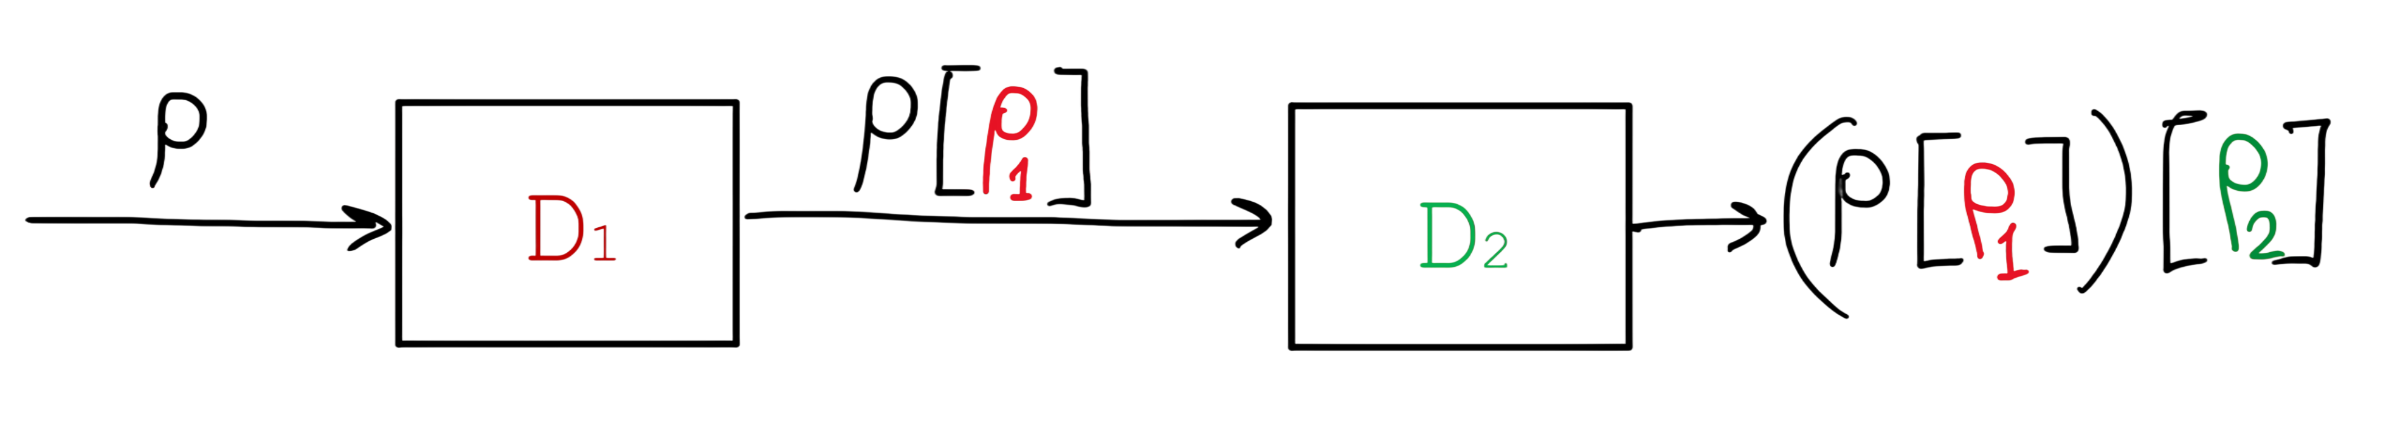
\includegraphics[width=0.5\textwidth]{images/composizione-sequenziale.png}
    \end{figure}

    \esempio{composizione sequenziale}{
        Consideriamo il seguente codice:
        \[
            \begin{aligned}
                &\texttt{const x: int = 3;} \\
                &\texttt{const x: int = 5;} && \texttt{const y: int = 6 * x;} \\
                &\texttt{const z: int = z + y;}
            \end{aligned}
        \]

        Osserviamo i valori che assumo le variabili di questo codice:
        \begin{enumerate}[itemsep=\smallskipamount]
            \item a riga 1 il valore assegnato a \texttt{x} è $\rho$ = [\texttt{x} $\mapsto$ \texttt{3}]
            \item a riga 2 il valore assegnato a \texttt{x} è $\rho_1$ = [\texttt{x} $\mapsto$ \texttt{5}] e viene usata per elaborare \texttt{y} che assume valore $\rho_2$ = [\texttt{y} $\mapsto$ \texttt{6 * 5 = 30}]
            \item a riga 3 viene usati il valore di \texttt{x} dichiarato a riga 2 e il valore di \texttt{y} dichiarato a riga 2 ($\rho_2$ = [\texttt{x} $\mapsto$ \texttt{5}, \texttt{y} $\mapsto$ \texttt{30}]) per elaborare \texttt{z} che assume il valore ($\rho_3$ = [\texttt{x} $\mapsto$ \texttt{5}, \texttt{y} $\mapsto$ \texttt{30}, \texttt{z} $\mapsto$ \texttt{5 + 30 = 35}])
        \end{enumerate}

        \begin{figure}[H]
            \centering
            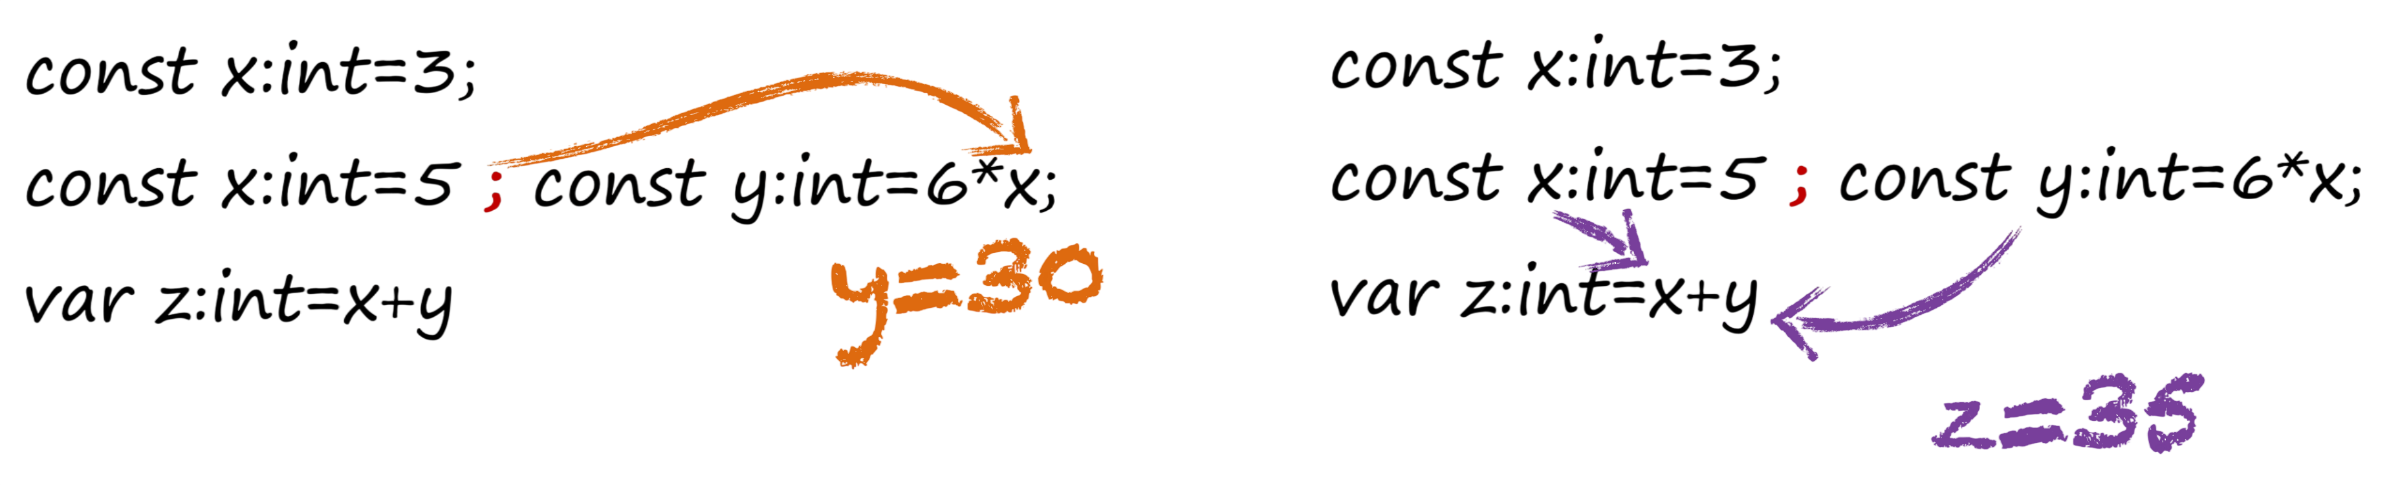
\includegraphics[width=0.6\textwidth]{images/esempio-composizione-sequenziale.png}
        \end{figure}
    }
    \item $\mathbf{D \ in \ D}$: composizione privata.
    
     I legami creati o sovrascritti da $\mathrm{D_1}$ sono ad uso esclusivo dell’elaborazione di $\mathrm{D_2}$ e non visibili al codice successivo

    \begin{figure}[H]
        \centering
        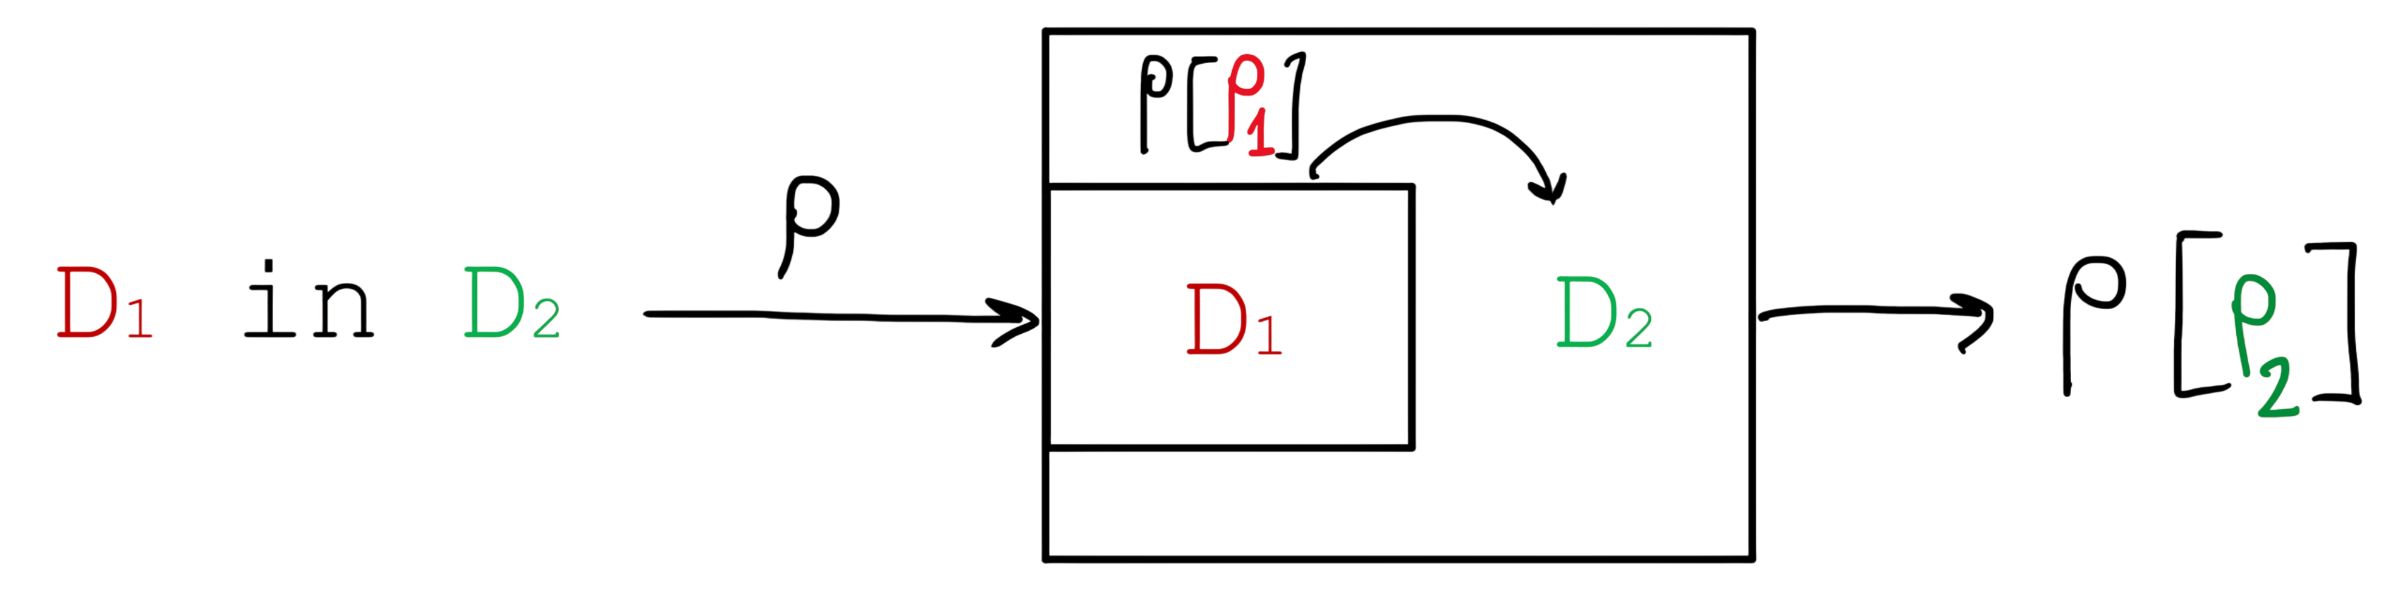
\includegraphics[width=0.5\textwidth]{images/composizione-privata.png}
    \end{figure}

    \esempio{composizione privata}{
        Consideriamo il seguente codice:
        \[
            \begin{aligned}
                &\texttt{const x: int = 3;} \\
                &\texttt{const x: int = 5;} && \texttt{const y: int = 6 * x;} \\
                &\texttt{const z: int = z + y;}
            \end{aligned}
        \]

        Osserviamo i valori che assumo le variabili di questo codice:
        \begin{enumerate}[itemsep=\smallskipamount]
            \item a riga 1 il valore assegnato a \texttt{x} è $\rho$ = [\texttt{x} $\mapsto$ \texttt{3}]
            \item a riga 2 il valore assegnato a \texttt{x} è $\rho_1$ = [\texttt{x} $\mapsto$ \texttt{5}] e viene usata per elaborare \texttt{y} che assume valore $\rho_2$ = [\texttt{y} $\mapsto$ \texttt{6 * 5 = 30}]
            \item a riga 3 viene usati il valore di \texttt{x} dichiarato a riga 1 e il valore di \texttt{y} dichiarato a riga 2 ($\rho_2$ = [\texttt{x} $\mapsto$ \texttt{5}, \texttt{y} $\mapsto$ \texttt{30}]) per elaborare \texttt{z} che assume il valore ($\rho_3$ = [\texttt{x} $\mapsto$ \texttt{5}, \texttt{y} $\mapsto$ \texttt{30}, \texttt{z} $\mapsto$ \texttt{3 + 30 = 33}])
        \end{enumerate}

        \begin{figure}[H]
            \centering
            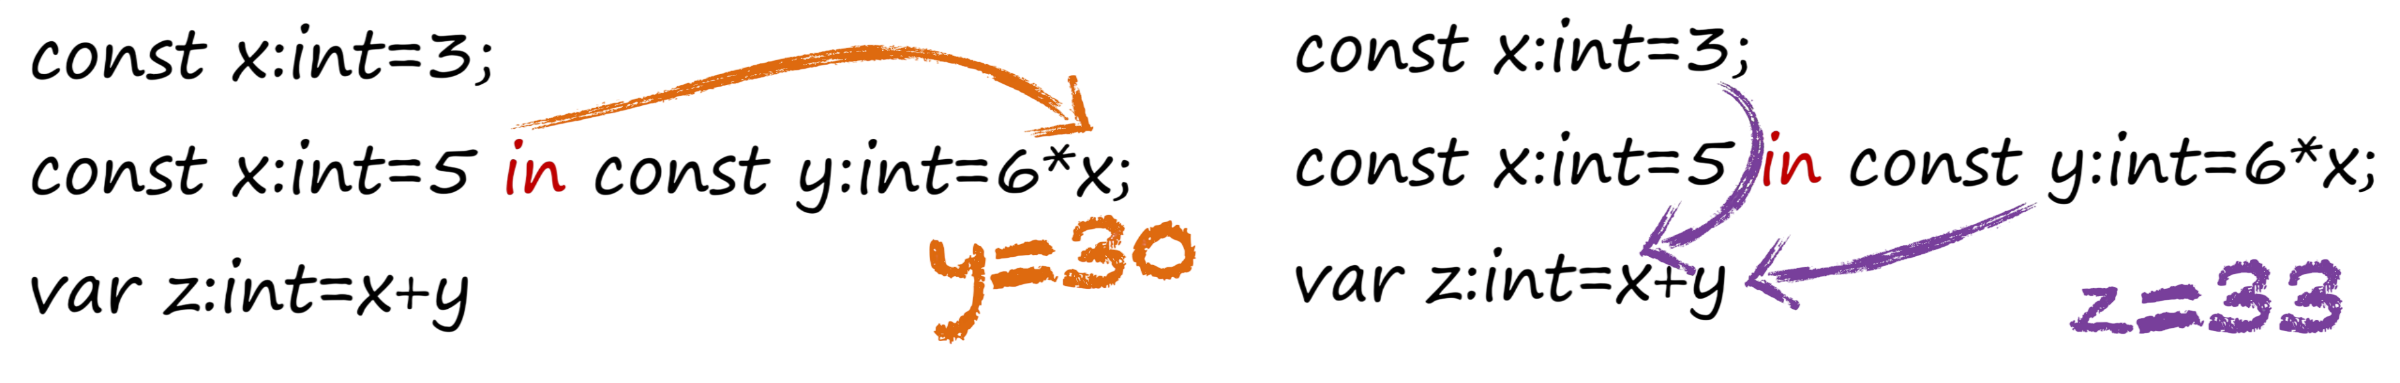
\includegraphics[width=0.6\textwidth]{images/esempio-composizione-privata.png}
        \end{figure}
    }
\end{itemize}

\subsection{Modifica dell'ambiente}
Consideriamo gli ambienti (dinamici):
\[
    \beta, \beta' \in \mathrm{Env} \quad \beta : V, \beta' : V' \quad V, V' \subseteq \mathrm{Id}
\]

La modifica di $\beta$ da parte di $\beta'$ si scrive:
\[
    \mathbf{\beta[\beta']}
\]

Il nuovo ambiente $\beta''$ (= $\beta[\beta']$) $\in \mathrm{Env}$ sarà:
\[
    \beta''(I) = 
    \begin{cases} 
        \beta'(I) & \text{se } I \in V \\
        \beta(I)  & \text{se } I \in V, V' 
    \end{cases}
\]

Ciò significa che parlerà sia degli identificatori in I che in quelli in I':
\[
    \beta[\beta'] = \hat{\beta} \ \hat{\beta}: I \cup I
\]

\esempio{modifica dell'ambiente}{
    Consideriamo i seguenti ambienti:
    \[
        \begin{aligned}
            \beta &= [\texttt{z} \mapsto \texttt{5}, y \mapsto \texttt{false}]\\
            \beta' &= [\texttt{x} \mapsto \texttt{3}, y \mapsto \texttt{true}]
        \end{aligned}
    \]

    La modifica di $\beta$ da parte di $\beta'$ è il seguente:
    \[
        \beta[\beta'] = [\texttt{x} \mapsto \texttt{5}, \texttt{y} \mapsto \texttt{true}]
    \]

    Il valore di \texttt{y} viene \textbf{sovrascritto} perchè è presente in entrambi gli ambienti.
}

\subsection{Identificatori definiti}
Gli identificatori definiti (da una dichiarazione) sono gli identificatori che trovano il significato associato dentro la dichiarazione.

\begin{mydef}{identificatore definito (formale)}
    Definiamo la funzione $\mathrm{DI}$ che associa ad ogni dichiarazione l'insieme degli identificatori:
    \[
        \mathbf{DI:} \ \mathbf{Dec} \rightarrow \mathcal{P}\mathbf{(Id)}
    \]

    \begin{itemize}[label=$\triangleright$, itemsep=\smallskipamount]
        \item $\mathrm{DI(\texttt{nil})} = \emptyset$
        \item $\mathrm{DI(\rho)} = \mathrm{V} \quad \rho : \mathrm{V}$ (attribuisce significato a tutti gli elementi del suo dominio)
        \item $\mathrm{DI(\texttt{const \ x:} \ \tau \texttt{ = e}) = \{\texttt{x}\}}$ (attribuisce significato all'identificatore che sta dichiarando)
        \item $\mathrm{DI(d_0 ; d_1) = DI(d_0) \cup DI(d_1)}$ (attribuisce significato a tutti gli identificatori a cui viene dato significato in $d_0$ e $d_1$)
        \item $\mathrm{DI(d_0 \texttt{ in } d_1) = DI(d_2)}$ (ciò che viene definito nella prima dichiarazione $d_1$ rimane privato e, quindi, non risulta legato all'esterno della composizione. 
        
        Fuori dalla composizione è legato solo ciò che viene definito nella seconda composizione $d_2$)
    \end{itemize}
\end{mydef}

\subsection{Identificatori liberi}
GLi identificatori liberi sono identificatori il cui significato va cercato esternamente (nel contesto) alla dichiarazione.

\begin{mydef}{identificatore libero (formale)}
    Definiamo la funzione $\mathrm{FI}$ che applicata ad una dichirazione restituisce l'insieme degli identificatori liberi nella dichiarazione:
    \[
        \mathbf{FI : dec} \rightarrow \mathcal{P}\mathbf{(Id)}
    \]

    \begin{itemize}[label=$\triangleright$, itemsep=\smallskipamount]
        \item $\mathrm{FI(\texttt{nil})} = \emptyset$
        \item $\mathrm{FI(\rho)} = \emptyset$
        \item $\mathrm{FI(\texttt{const \ x:} \ \tau \texttt{ = e}) = FI(\texttt{e})}$
        \item $FI(d_0 ; d_1) = FI(d_1 \text{ in } d_2) = FI(d_1) \cup (FI(d_2) \underbrace{\setminus}_{\textcolor{red}{\text{togliere}}} DI(d_1))$
    \end{itemize}
\end{mydef}

\section{Semantica}

\subsection{Semantica statica}
\begin{mydef}{semantica statica}
    La \textbf{semantica statica} verifica se una dichiarazione è ben formata (rispetta vincoli contestuali).
\end{mydef}

La semantica statica per per dichiarazioni associa un ambiente statico $\Delta$ ad ogni dichiarazione ben formata.\\[0.2ex]
Le regole hanno la seguente forma:
\[
    \mathbf{D_{S_I}:} \ \textcolor{red}{\mathbf{\Delta \vdash_\mathbf{V}}} \ \mathbf{d : \Delta}
\]


Vediamo, quindi, le regole:
\begin{itemize}[label=$\triangleright$, itemsep=\smallskipamount]
    \item \textbf{regola 1} (assioma per gli ambienti statici):
    \vario{Assioma $\mathcal{D}_{\mathrm{S_1}}$}{
        \[
            \mathcal{D}_{\mathrm{S_1}}: \vdash \texttt{nill} : \emptyset
        \]
    }
    \item \textbf{regola 2} (assioma per gli ambienti dinamici):
    \item \vario{Assioma $\mathcal{D}_{\mathrm{S_2}}$}{
        \[
            \mathcal{D}_{\mathrm{S_2}}: \vdash \rho : \Delta \quad \Leftrightarrow \quad \rho \vdash \Delta
        \]
    }
    \item \textbf{regola 3}:
    \vario{Regola $\mathcal{D}_{\mathrm{S_3}}$}{
        \[
            \mathcal{D}_{\mathrm{S_3}}:\;
            \begin{prooftree}
                \hypo{\Delta \vdash_V e : \tau}
                \infer1{\Delta \vdash_V \texttt{const x:} \ \tau \texttt{ = e}: [\texttt{x} \gets \tau]}
            \end{prooftree}
        \]
    }
    \item \textbf{regola 4} (dichiarazione composta):
    \vario{Regola $\mathcal{D}_{\mathrm{S_4}}$}{
        \[
            \mathcal{D}_{\mathrm{S_4}}:\;
            \begin{prooftree}
                \hypo{\Delta \vdash d_1 : \Delta_1 \quad \Delta_1[\Delta_2] \vdash d_2 : \Delta_2}
                \infer1{\Delta \vdash d_1 ; d_2 : \Delta_1[\Delta_2]}
            \end{prooftree}
        \]
    }
    \item \textbf{regola 5} (dichiarazione composta):
    \vario{Regola $\mathcal{D}_{\mathrm{S_5}}$}{
        \[
            \mathcal{D}_{\mathrm{S_5}}:\;
            \begin{prooftree}
                \hypo{\Delta \vdash d_1 : \Delta_1 \quad \Delta_1[\Delta_2] \vdash d_2 : \Delta_2}
                \infer1{\Delta \vdash d_1 \texttt{ in } d_2 : \Delta_2}
            \end{prooftree}
        \]
    }
\end{itemize}

\subsection{Semantica dinamica}
\begin{mydef}{semantica dinamica}
    La \textbf{semantica dinamica} consiste nell'elaborazione che parte dall'assunzione che la dichiarazione è ben formata.
\end{mydef}

Le regole di transizione hanno la forma:
\[
    \mathcal{D}_\mathbf{i} : \rho \ \textcolor{red}{\mathbf{\vdash_\Delta}} \ \mathbf{d} \to_\mathrm{d} \mathbf{d'}
\]

dove:
\begin{itemize}[label=$\triangleright$, itemsep=\smallskipamount]
    \item $\rho$: ambiente nel quale elaboriamo la dichiarazione (compatibile con $\Delta$)
    \item $\mathrm{d}$: dichiarazione che viene elaborata in $\mathrm{d}'$ nell'ambiente $\rho$
\end{itemize}

Vediamo, quindi, le regole:
\begin{itemize}[label=$\triangleright$, itemsep=\smallskipamount]
    \item \textbf{regola 1} (assioma): $\rho$ è già terminale (non c'è nulla da elaborare)
    \vario{Assioma $\mathcal{D}_{\mathrm{S_1}}$}{
        \[
            \mathcal{D}_1 : \ \vdash \texttt{nil} \to_d \emptyset
        \]
    }
    \item \textbf{regola 2} (assioma):
    \vario{Assioma $\mathcal{D}_{\mathrm{S_2}}$}{
        \[
            \mathcal{D}_2 : \rho \ \vdash \texttt{const x:} \ \tau \texttt{ = k} \to_d [x \mapsto k]
        \]
    }
    \item \textbf{regola 3}:
    \vario{Regola $\mathcal{D}_{\mathrm{S_3}}$}{
        \[
            \mathcal{D}_3:\;
            \begin{prooftree}
                \hypo{\rho \vdash\Delta e \to_e e'}
                \infer1{\rho \vdash_\Delta \texttt{const x:} \ \tau \texttt{ = e} \to_d \texttt{const x:} \ \tau \texttt{ = e'}}
            \end{prooftree}
        \]
    }
    \item \textbf{regola 4}:
    \vario{Regola $\mathcal{D}_{\mathrm{S_4}}$}{
        \[
            \mathcal{D}_4:\;
            \begin{prooftree}
                \hypo{\rho \vdash\Delta d \to_e d'}
                \infer1{\rho \vdash_\Delta d ; d_1 \to_d d' ; d_1}
            \end{prooftree}
        \]
    }
    \item \textbf{regola 5}:
    \vario{Regola $\mathcal{D}_{\mathrm{S_5}}$}{
        \[
            \mathcal{D}_5:\;
            \begin{prooftree}
                \hypo{\rho[\rho_0] \vdash\Delta d_1 \to_e d_1'}
                \infer1{\rho \vdash_\Delta \rho_0 ; d_1 \to_d \rho_0 ; d_1'}
            \end{prooftree}
        \]
    }
    \item \textbf{regola 6}:
    \vario{Regola $\mathcal{D}_{\mathrm{S_6}}$}{
        \[
            \mathcal{D}_6: \rho \vdash_\Delta \rho_0 ; \rho_1 \to_d \rho_0[\rho_1]
        \]
    }
    \item \textbf{regola 7}:
    \vario{Regola $\mathcal{D}_{\mathrm{S_7}}$}{
        \[
            \mathcal{D}_7:\;
            \begin{prooftree}
                \hypo{\rho \vdash\Delta d \to_e d'}
                \infer1{\rho \vdash_\Delta d \texttt{ in } d_1 \to_d d \texttt{ in } d_1}
            \end{prooftree}
        \]
    }
    \item \textbf{regola 8}:
    \vario{Regola $\mathcal{D}_{\mathrm{S_8}}$}{
        \[
            \mathcal{D}_8:\;
            \begin{prooftree}
                \hypo{\rho[\rho_0] \vdash\Delta d_1 \to_e d_1'}
                \infer1{\rho \vdash_\Delta \rho_0 \texttt{ in } d_1 \to_d \rho_0 \texttt{ in } d_1'}
            \end{prooftree}
        \]
    }
    \item \textbf{regola 9}:
    \vario{Regola $\mathcal{D}_{\mathrm{S_9}}$}{
        \[
            \mathcal{D}_9: \rho \vdash_\Delta \rho_0 \texttt{ in } \rho_1 \to_d \rho_0[\rho_1]
        \]
    }
\end{itemize}

\begin{mydef}{elaborazione delle dichiarazioni}
    La \textbf{valutazione} è una funzione
    \[
        \mathbf{Elab:} \mathcal{D} \to \mathbf{Env}
    \]

    che descrive il comportamento dinamico delle dichiarazioni restituendo l'ambiente in cui esse sono elaborate:
    \[
        \mathrm{Elab(d)} = \rho \quad \Leftrightarrow \quad \to * \rho
    \]
\end{mydef}

La definizione di valutazione di una dichiarazione permette, anche, di definire il concetto di equivalenza tra dichiarazioni.

\begin{mydef}{equivalenza di dichiarazioni}
    L'\textbf{equivalenza di dichiarazioni} è una relazione
    \[
        \equiv \ \subseteq \mathcal{D} \times \mathcal{D}
    \]

    definita come segue:
    \[
        d_0 \equiv d_1 \quad \Leftrightarrow \quad \mathrm{Elab(d_0) = Elab(d_1)}
    \]
\end{mydef}